\documentclass[aspectratio=1610,mathserif]{beamer}
\usepackage{tikz}
\usetikzlibrary{shapes,decorations,arrows,positioning,fit}
\tikzset{point/.style={circle,draw,fill=csmblue,radius=2pt}}
\tikzset{cpoint/.style={circle,draw,fill=csmred,radius=2pt}}
\tikzset{>=stealth',thick,color=csmblue}

\usetheme{csam}

\title{Multi-Agent Continuous Motion Simulation using Discrete Events}
\author{Jack Rosenthal and Qin Yang}
\institute{Robot Planning \& Manipulation}

\begin{document}

\maketitle

\begin{frame}{Background on Discrete Event Simulation}
    Computer simulations come in different varieties:
    \begin{itemize}
        \item \textbf{Monte-Carlo Simulations:} Simulating events which do not
            occur over a period of time, or where time is not important. For
            example, rolling a 6-sided die 1000 times.
        \item \textbf{Time-Step Simulations:} Simulating a system for which
            time is important; system clock is incremented by a fixed value for
            each time step, and the next state of the system is computed. For
            example, Conway's Game of Life.
        \item \textbf{Discrete Event Simulations:} Simulating a system for
            which time is important, but \emph{the clock is not incremented by
            a fixed amount}, instead, we define the system using events and
            skip to the next event each time.
    \end{itemize}
\end{frame}

\begin{frame}{What simulation techniques are used in robotics?}
    Currently, all robotics simulation frameworks we could find use a time-step
    model (ARGoS, Gazebo, USARSim, Webots, MuRoSimF).

    What if there was a way to use DES to simulate multi-robot systems?
\end{frame}

\begin{frame}{Problem Statement}
    Given $N$-agents in a $k$-dimensional system, how can we develop a
    simulation technique to model the motion of the agents in a continuous
    space without resorting to time-step?
\end{frame}

\begin{frame}{Cross-Cutting and Cancellation}
    \begin{columns}
        \begin{column}{0.4\textwidth}
            \begin{tikzpicture}
                \node[point,label=below:{$A$}] (Ainitial) at (0,0) {};
                \node[point,label=above left:{$E_{B1}$}] (collide) at (2,2) {};
                \node[cpoint,label={$E_{A1}$}] (EA1) at (4,4) {};
                \node[point,label={$E_{A2}$}] (EA2) at (4,2) {};

                \node[point,label=below:{$B$}] (Binitial) at (3,0) {};
                \node[point,label={$E_{B2}$}] (EB2) at (2,4) {};

                \draw (Ainitial) -- (collide) node[midway,sloped,below] {$f_{A1}(t)$};
                \draw[->,dashed] (collide) -- (EA1) node[midway,sloped,above] {$f_{A1}(t)$};
                \draw[->] (collide) -- (EA2) node[midway,sloped,above] {$f_{A2}(t)$};
                \draw[->] (Binitial) -- (EB2) node[near start,sloped,below] {$f_{B1}(t)$};
            \end{tikzpicture}
        \end{column}
        \begin{column}{0.6\textwidth}
            In order to prevent collision, we need to be clever with how we
            process each event. We extend the traditional DES model in two ways:
            \begin{itemize}
                \item \textbf{Cross-cutting} functions are computed each time a
                    simulation agent makes a travel plan. This is a continuous
                    function which can be symbolically manipulated.
                \item \textbf{Cancellation} allows events to be cancelled from
                    when they were originally scheduled, and allows us to have
                    agents make an initial plan that then changes.
            \end{itemize}
        \end{column}
    \end{columns}
\end{frame}

\begin{frame}{Evaluation}
    In order to evaluate the feasibility of our simulation technique, we
    implemented the simulation in a simple multi-agent robotics scenario:

    \begin{itemize}
        \item When a task (shown in red) is added, the robots divide and work
            on the task.
        \item Two tasks added close together may cause cancellation.
    \end{itemize}

    \begin{columns}
        \begin{column}{0.33\textwidth}
            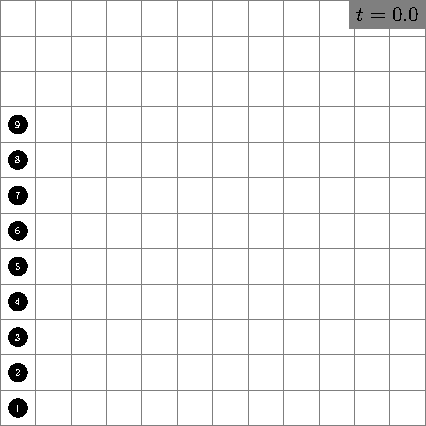
\includegraphics[width=\textwidth]{sim1.pdf}
        \end{column}
        \begin{column}{0.33\textwidth}
            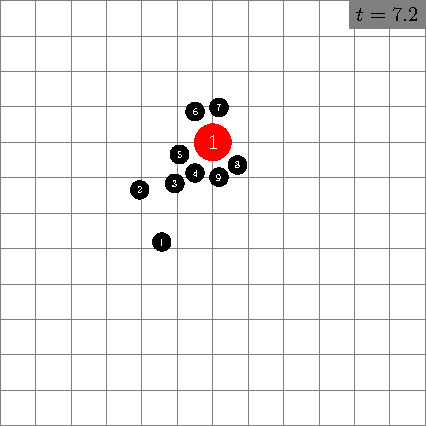
\includegraphics[width=\textwidth]{sim73.pdf}
        \end{column}
        \begin{column}{0.33\textwidth}
            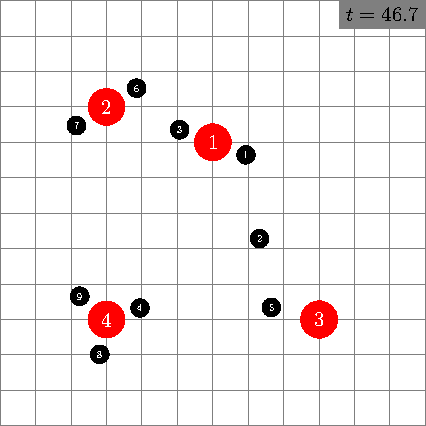
\includegraphics[width=\textwidth]{sim468.pdf}
        \end{column}
    \end{columns}
\end{frame}

\begin{frame}{Tradeoffs of DES for Multi-Agent Planning Simulations}
    \begin{itemize}
        \item \textbf{Advantage:} Decreased computational time needed to run
            simulation on many agents, especially when events are spaced far
            apart.
        \item \textbf{Disadvantage:} Implementing and verifying the simulation
            becomes much more difficult, as special care must be taken to use
            the cross cutting functions correctly.
        \item \textbf{Disadvantage:} When a large number of cancellations
            occurs, the event queue grows quite large, and increases
            computational time. Care must either be taken to use cancellation
            where appropriate, or use cancellation-elimination algorithms.
    \end{itemize}
\end{frame}

\end{document}
